\documentclass[
	9pt, % Set the default font size, options include: 8pt, 9pt, 10pt, 11pt, 12pt, 14pt, 17pt, 20pt
	t, % Uncomment to vertically align all slide content to the top of the slide, rather than the default centered
	%aspectratio=169, % Uncomment to set the aspect ratio to a 16:9 ratio which matches the aspect ratio of 1080p and 4K screens and projectors
]{beamer}

\graphicspath{{Images/}{./}} % Specifies where to look for included images (trailing slash required)

\usepackage{booktabs} % Allows the use of \toprule, \midrule and \bottomrule for better rules in tables
\usepackage{graphicx}
\usepackage{caption}
\usepackage{subcaption}
\usepackage{hyperref}
\usepackage[english,brazil]{babel}
\usepackage{fontawesome5}
\usepackage{listings}
\usepackage{minted}
\usepackage{xcolor}
% \usepackage{graphicx}
% \usepackage{animate}
\RequirePackage[backend=biber,
style=ieee,
citestyle=authoryear,
]{biblatex}

% Define a custom command for an icon link
\newcommand{\iconLink}[2]{\href{#1}{\faLink \hspace{0.2em} {#2}}}
\newcommand{\yellowbox}[1]{\colorbox{yellow!75}{#1}}

% Definindo um estilo para o destaque
%----------------------------------------------------------------------------------------
%	SELECT LAYOUT THEME
%----------------------------------------------------------------------------------------
\usetheme{Madrid}

%----------------------------------------------------------------------------------------
%	SELECT COLOR THEME
%----------------------------------------------------------------------------------------

% Beamer comes with a number of color themes that can be applied to any layout theme to change its colors. Uncomment each of these in turn to see how they change the colors of your selected layout theme.

%\usecolortheme{albatross}
%\usecolortheme{beaver}
%\usecolortheme{beetle}
% \usecolortheme{crane}
%\usecolortheme{dolphin}
%\usecolortheme{dove}
%\usecolortheme{fly}
%\usecolortheme{lily}
%\usecolortheme{monarca}
%\usecolortheme{seagull}
%\usecolortheme{seahorse}
%\usecolortheme{spruce}
%\usecolortheme{whale}
%\usecolortheme{wolverine}

%----------------------------------------------------------------------------------------
%	SELECT FONT THEME & FONTS
%----------------------------------------------------------------------------------------
\usefonttheme{default} % Typeset using the default sans serif font

%------------------------------------------------

\usepackage{palatino} % Use the Palatino font for serif text
\usepackage[default]{lato} % Use the Lato font for sans serif text

%----------------------------------------------------------------------------------------
%	SELECT INNER THEME
%----------------------------------------------------------------------------------------
\useinnertheme{rectangles}

%----------------------------------------------------------------------------------------
%	SELECT OUTER THEME
%----------------------------------------------------------------------------------------

% Outer themes change the overall layout of slides, such as: header and footer lines, sidebars and slide titles. Uncomment each theme in turn to see what changes it makes to your presentation.

%\useoutertheme{default}
%\useoutertheme{infolines}
%\useoutertheme{miniframes}
%\useoutertheme{smoothbars}
%\useoutertheme{sidebar}
%\useoutertheme{split}
%\useoutertheme{shadow}
%\useoutertheme{tree}
%\useoutertheme{smoothtree}

%\setbeamertemplate{footline} % Uncomment this line to remove the footer line in all slides
%\setbeamertemplate{footline}[page number] % Uncomment this line to replace the footer line in all slides with a simple slide count

%\setbeamertemplate{navigation symbols}{} % Uncomment this line to remove the navigation symbols from the bottom of all slides

% \bibliography{references} % Specifies the bibliography file to include publications
% \bibliographystyle{apalike} % Specifies the bibliography style
\addbibresource{references.bib}

%----------------------------------------------------------------------------------------
%	PRESENTATION INFORMATION
%----------------------------------------------------------------------------------------

\title[DesWebII]{Desenvolvimento Web II} % The short title in the optional parameter appears at the bottom of every slide, the full title in the main parameter is only on the title page
\subtitle{Aula 06 - Integração e Entrega Contínua - CI/CD} % Presentation subtitle, remove this command if a subtitle isn't required
\author[Fabricio Bizotto]{Prof. Fabricio Bizotto} % Presenter name(s), the optional parameter can contain a shortened version to appear on the bottom of every slide, while the main parameter will appear on the title slide
\institute[IFC]{Instituto Federal Catarinense \\ \smallskip \textit{fabricio.bizotto@ifc.edu.br}} % Your institution, the optional parameter can be used for the institution shorthand and will appear on the bottom of every slide after author names, while the required parameter is used on the title slide and can include your email address or additional information on separate lines
\date[\today]{Ciência da Computação \\ \today} % Presentation date or conference/meeting name, the optional parameter can contain a shortened version to appear on the bottom of every slide, while the required parameter value is output to the title slide

%----------------------------------------------------------------------------------------
\begin{document}

%----------------------------------------------------------------------------------------
%	TITLE SLIDE
%----------------------------------------------------------------------------------------

\begin{frame}
	\titlepage % Output the title slide, automatically created using the text entered in the PRESENTATION INFORMATION block above
\end{frame}

%----------------------------------------------------------------------------------------
%	TABLE OF CONTENTS SLIDE
%----------------------------------------------------------------------------------------

\begin{frame}
	\frametitle{Roteiro} % Slide title, remove this command for no title
	
	\tableofcontents % Output the table of contents (all sections on one slide)
	%\tableofcontents[pausesections] % Output the table of contents (break sections up across separate slides)
\end{frame}

%----------------------------------------------------------------------------------------
%	PRESENTATION BODY SLIDES
%----------------------------------------------------------------------------------------

\section{Manifesto Ágil}

%------------------------------------------------

\begin{frame}
	\frametitle{Manifesto Ágil}
	\begin{itemize}
		\item O Manifesto Ágil foi escrito em 2001 por 17 desenvolvedores de software que se reuniram para discutir métodos leves de desenvolvimento de software.
		\item O Manifesto Ágil é baseado em 4 valores e 12 princípios.
		\item Os 4 valores do Manifesto Ágil são:
		\begin{enumerate}
			\item Indivíduos e interações mais que processos e ferramentas;
			\item Software em funcionamento mais que documentação abrangente;
			\item Colaboração com o cliente mais que negociação de contratos;
			\item Responder a mudanças mais que seguir um plano.
		\end{enumerate}
	\end{itemize}
\end{frame}

\section{Integração Contínua} % Sections are added in order to organize your presentation into discrete blocks, all sections and subsections are automatically output to the table of contents as an overview of the talk but NOT output in the presentation as separate slides

%------------------------------------------------

\begin{frame}
	\frametitle{Integração Contínua - \textit{Continuous Integration (CI)}}
	\begin{itemize}
		\item CI é uma \yellowbox{prática} de desenvolvimento de software em que os desenvolvedores integram \yellowbox{pequenos pedaços} de código em um repositório compartilhado \yellowbox{frequentemente}, de preferência várias vezes ao dia.
		\item Cada integração é verificada por uma \yellowbox{\textbf{build} automatizada} (incluindo testes) para detectar erros de integração o mais rápido possível.
		\item Esse tipo de abordagem leva a uma redução significativa nos problemas de integração e permite que uma equipe desenvolva software coeso mais rapidamente.
		\item O CI pode ser falhar por: \textbf{builds} quebradas, testes quebrados, cobertura de testes insuficiente, etc.
	\end{itemize}

	\begin{block}{Pipeline - Fluxo de Trabalho}
		\begin{enumerate}
			\item \textbf{Controle de Versão}: Desenvolvedor faz \textbf{commit} no repositório compartilhado;
			\item \textbf{Gatilho Automático}: Servidor de CI monitora o repositório e faz o \textbf{pull} do código;
			\item \textbf{Compilação e Testes Automatizados}: Servidor de CI executa a \textbf{build} e os testes;
			\item \textbf{Relatório}: Servidor de CI notifica o desenvolvedor sobre o resultado. 
		\end{enumerate}
	\end{block}

\end{frame}

%------------------------------------------------

\begin{frame}
	\frametitle{Integração Contínua}
	\begin{figure}
		\centering
		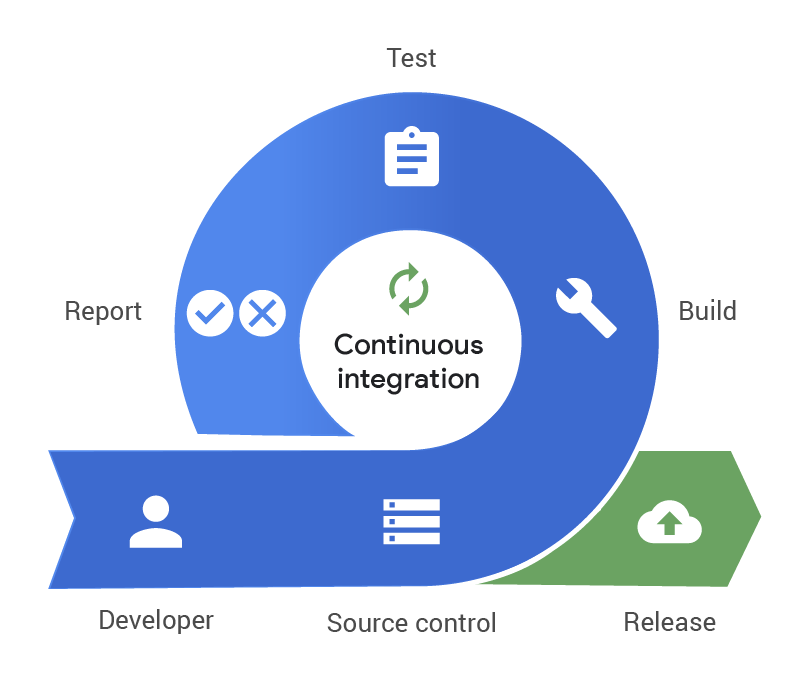
\includegraphics[width=0.7\linewidth]{cont_integ.png}
		\caption{Integração Contínua}
		\label{fig:ci}
	\end{figure}

\end{frame}

%------------------------------------------------

\section{Entrega Contínua}

%------------------------------------------------

\begin{frame}
	\frametitle{Entrega Contínua - \textit{Continuous Delivery (CD)}}
	\begin{itemize}
		\item CD é uma abordagem de engenharia de software na qual as equipes produzem software em ciclos curtos, garantindo que o software possa ser implantado de forma confiável a qualquer momento.
		\item Com o CD, o código é sempre implantável, desde o início do projeto.
		\item O CD visa tornar o processo de implantação automatizado, de modo que qualquer alteração no software possa ser implantada de forma rápida e segura.
		\item O CD pode ser falhar por: \textbf{builds} quebradas, testes quebrados, cobertura de testes insuficiente, etc.
	\end{itemize}

	\begin{block}{Fluxo de Trabalho}
		\begin{enumerate}
			\item \textbf{Controle de Versão}: Desenvolvedor faz \textbf{commit} no repositório compartilhado;
			\item \textbf{Gatilho Automático}: Servidor de CI monitora o repositório e faz o \textbf{pull} do código;
			\item \textbf{Compilação e Testes Automatizados}: Servidor de CI executa a \textbf{build} e os testes;
			\item \textbf{Implantação Automatizada}: Servidor de CI implanta o código em um ambiente de teste;
			\item \textbf{Relatório}: Servidor de CI notifica o desenvolvedor sobre o resultado. 
		\end{enumerate}
	\end{block}

\end{frame}
	
\end{document} 
